\documentclass[12pt]{article}
\usepackage[utf8]{inputenc}
\usepackage{float}
\usepackage{amsmath}
\hbadness=10000

\usepackage[hmargin=3cm,vmargin=6.0cm]{geometry}
%\topmargin=0cm
\topmargin=-2cm
\addtolength{\textheight}{6.5cm}
\addtolength{\textwidth}{2.0cm}
%\setlength{\leftmargin}{-5cm}
\setlength{\oddsidemargin}{0.0cm}
\setlength{\evensidemargin}{0.0cm}

%misc libraries goes here
\usepackage{tikz}
\usetikzlibrary{automata,positioning}

\begin{document}

\section*{Student Information } 
%Write your full name and id number between the colon and newline
%Put one empty space character after colon and before newline
Full Name :  Yasin Fatih ALPUL\\
Id Number :  2098739\\

% Write your answers below the section tags
\section*{Answer 1}

\subsection*{a.}
We know that $A$ is countably infinite or finite if $B$ is countably infinite given $A$ is a subset of $B$. ($A \subseteq B$). Also, set of rational numbers on interval $(-1,0)$ is a subset of all rational numbers on $(-\infty,\infty)$ interval. If we show that rational numbers on that interval are countable, then, so are rational numbers on $(-1,0)$.\\
We can define\\
$$Q = \left\{\frac{a}{b} ~~\text{such that}~~(a,b) \in Z\times Z\right\}$$
$Z$ is countable, as an enumeration can be given such as $Z=\{0,1,-1,2,-2,\dots \}$, since product of two countable sets is countable, as it can be enumerated while alternating (i.e dovetailing), then $Q$ is countable.\\
In addition, we can divide the interval $(-1,0)$ to arbitrarily small pieces, thus making the set infinite. Hence, the set of rational numbers inside the open interval $(-1,0)$ is countable and infinite.
\subsection*{b.}
The set is defined to be requiring these two properties.
\begin{itemize}
    \item $L$ is a finite language over the unary alphabet $\sum = \{a\}$
    \item $L^+$ is not regular
\end{itemize}
Let $K$ be any language, $K^+$ is defined as $K\circ K^*$ where $\circ$ is the concatenation operator and $*$ is the Kleene Star. Both operations are closed for regular languages. Moreover, union operator is also closed for regular languages. $L$ is given as a finite language where language is defined as a set of words. Any single word is a regular expression. That is, a word is merely a concatenation$(\circ)$ of symbols in the alphabet which is closed for regular languages as mentioned. Union for these words is regular and so is $L^+$ by successively applying the operators closed for regular languages.\\~\\
The set also requires $L^+$ to be not regular. The empty set$(\emptyset)$ is the only set meeting that requirement. As $D$ being empty, that makes it countable and finite.
\\~\\
\subsection*{c.}
The set of all languages on the binary alphabet $\sum = \{a,b\}$ consists of the following two sets:
\begin{enumerate}
    \item The set of all languages that can be recognized by a finite automaton
    \item The set of all languages that cannot be recognized by a finite automaton
\end{enumerate}
The first set is countable\textbf{(*)}, we also know that union of two countable sets is countable. However, the set of all languages on the binary alphabet $\sum = \{a,b\}$ is not countable \textbf{(**)}, therefore, the set of all languages that cannot be recognized by a finite automaton is uncountable and infinite.\\~\\
\indent \textbf{(*)} Every regular language is recognized by some deterministic finite automaton. Moreover, the description of each DFA is also finite. We can describe their states, transitions etc. in a standard finite way. So we can order these automata by their increasing length. This leads to a bijection on $N$ thus making it countable.\\~\\
\indent \textbf{(**)} Taking the advantage of Cantor's Diagonalization Argument, since languages are subsets of $\sum^*$ and strings generated from $\sum = \{a,b\}$ are countably infinite (order by their increasing length), its subsets are uncountable. This can be seen by creating a bijection to $N$ and showing that $2^N$ is uncountable. Let there be an enumeration such as $\{a,b,aa,ab,ba,bb...\}$ we see that this is a $1-to-1$ correspondence to $N$. Assume $2^N$ is countable, then we can set an enumeration such as $\{a_1,a_2,a_3..\}$ and let $B=\{i \in N~ |~ i \notin a_i\}$ (which is a valid set), then by diagonalization we could find an $a_j$ which is not in the enumeration. Hence, the assumption was incorrect and $2^N$ is uncountable.\\
Therefore, the set of all languages that cannot be recognized by a finite automaton is uncountable and infinite.
\section*{Answer 2}
\subsection*{a.}

\begin{center}
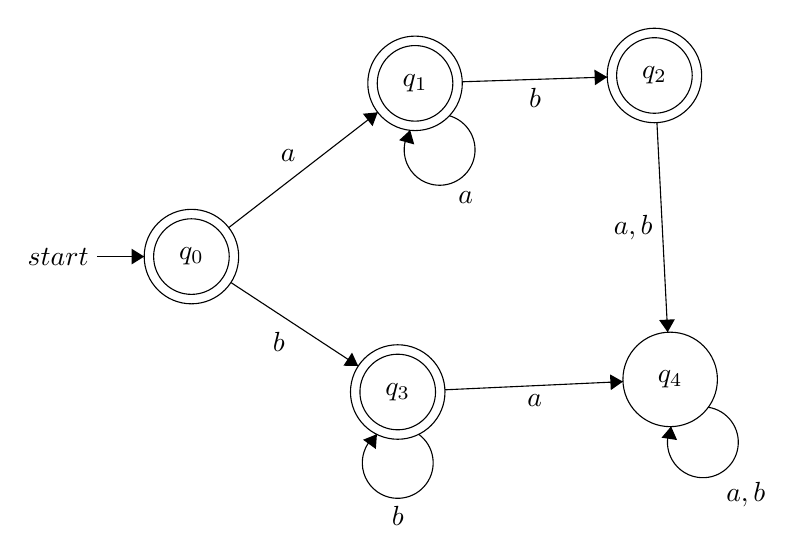
\begin{tikzpicture}[scale=0.2]
\tikzstyle{every node}+=[inner sep=0pt]
\draw [black] (13.6,-29.5) circle (3);
\draw (13.6,-29.5) node {$q_0$};
\draw [black] (13.6,-29.5) circle (2.4);
\draw [black] (27.8,-18.5) circle (3);
\draw (27.8,-18.5) node {$q_1$};
\draw [black] (27.8,-18.5) circle (2.4);
\draw [black] (26.7,-38.1) circle (3);
\draw (26.7,-38.1) node {$q_3$};
\draw [black] (26.7,-38.1) circle (2.4);
\draw [black] (43,-18) circle (3);
\draw (43,-18) node {$q_2$};
\draw [black] (43,-18) circle (2.4);
\draw [black] (44,-37.3) circle (3);
\draw (44,-37.3) node {$q_4$};
\draw [black] (15.97,-27.66) -- (25.43,-20.34);
\fill [black] (25.43,-20.34) -- (24.49,-20.43) -- (25.1,-21.22);
\draw (19.75,-23.5) node [above] {$a$};
\draw [black] (16.11,-31.15) -- (24.19,-36.45);
\fill [black] (24.19,-36.45) -- (23.8,-35.6) -- (23.25,-36.43);
\draw (19.15,-34.3) node [below] {$b$};
\draw [black] (28.023,-40.78) arc (54:-234:2.25);
\draw (26.7,-45.35) node [below] {$b$};
\fill [black] (25.38,-40.78) -- (24.5,-41.13) -- (25.31,-41.72);
\draw [black] (29.969,-20.555) arc (74.28256:-213.71744:2.25);
\draw (31.02,-25.36) node [below] {$a$};
\fill [black] (27.49,-21.47) -- (26.79,-22.11) -- (27.75,-22.38);
\draw [black] (29.7,-37.96) -- (41,-37.44);
\fill [black] (41,-37.44) -- (40.18,-36.98) -- (40.23,-37.98);
\draw (35.39,-38.24) node [below] {$a$};
\draw [black] (30.8,-18.4) -- (40,-18.1);
\fill [black] (40,-18.1) -- (39.19,-17.63) -- (39.22,-18.62);
\draw (35.42,-18.78) node [below] {$b$};
\draw [black] (43.16,-21) -- (43.84,-34.3);
\fill [black] (43.84,-34.3) -- (44.3,-33.48) -- (43.3,-33.53);
\draw (42.92,-27.67) node [left] {$a,b$};
\draw [black] (46.41,-39.067) arc (81.47986:-206.52014:2.25);
\draw (48.8,-43.79) node [below] {$a,b$};
\fill [black] (44.06,-40.29) -- (43.45,-41) -- (44.44,-41.15);
\draw [black] (7.6,-29.5) -- (10.6,-29.5);
\draw (7.1,-29.5) node [left] {$start$};
\fill [black] (10.6,-29.5) -- (9.8,-29) -- (9.8,-30);
\end{tikzpicture}
\end{center}

\subsection*{b.}


\begin{center}
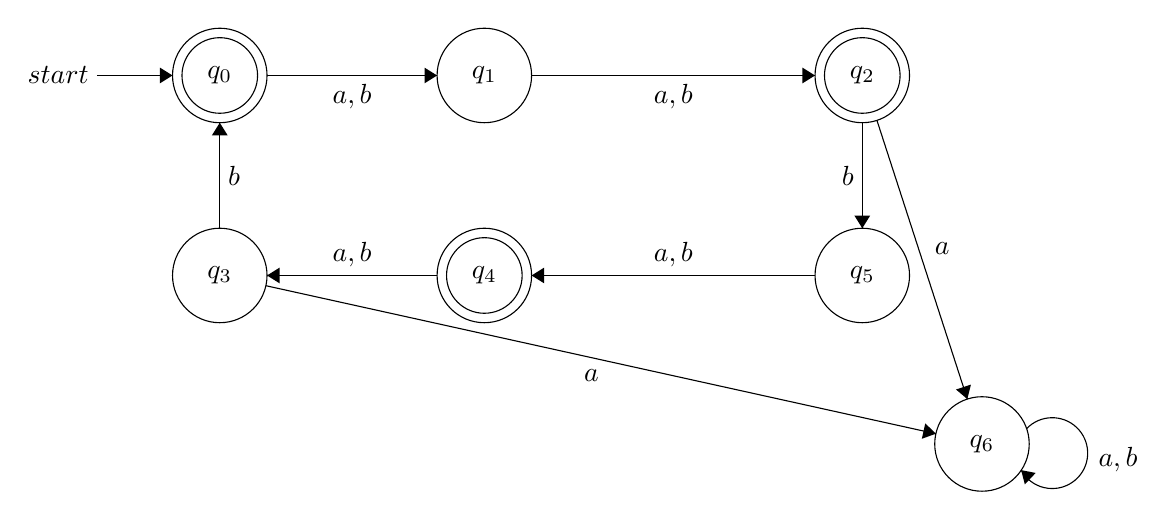
\begin{tikzpicture}[scale=0.2]
\tikzstyle{every node}+=[inner sep=0pt]
\draw [black] (15.2,-5.7) circle (3);
\draw (15.2,-5.7) node {$q_0$};
\draw [black] (15.2,-5.7) circle (2.4);
\draw [black] (32,-5.7) circle (3);
\draw (32,-5.7) node {$q_1$};
\draw [black] (56,-5.7) circle (3);
\draw (56,-5.7) node {$q_2$};
\draw [black] (56,-5.7) circle (2.4);
\draw [black] (15.2,-18.4) circle (3);
\draw (15.2,-18.4) node {$q_3$};
\draw [black] (32,-18.4) circle (3);
\draw (32,-18.4) node {$q_4$};
\draw [black] (32,-18.4) circle (2.4);
\draw [black] (56,-18.4) circle (3);
\draw (56,-18.4) node {$q_5$};
\draw [black] (63.6,-29.1) circle (3);
\draw (63.6,-29.1) node {$q_6$};
\draw [black] (18.2,-5.7) -- (29,-5.7);
\fill [black] (29,-5.7) -- (28.2,-5.2) -- (28.2,-6.2);
\draw (23.6,-6.2) node [below] {$a,b$};
\draw [black] (35,-5.7) -- (53,-5.7);
\fill [black] (53,-5.7) -- (52.2,-5.2) -- (52.2,-6.2);
\draw (44,-6.2) node [below] {$a,b$};
\draw [black] (56,-8.7) -- (56,-15.4);
\fill [black] (56,-15.4) -- (56.5,-14.6) -- (55.5,-14.6);
\draw (55.5,-12.05) node [left] {$b$};
\draw [black] (56.93,-8.55) -- (62.67,-26.25);
\fill [black] (62.67,-26.25) -- (62.9,-25.33) -- (61.95,-25.64);
\draw (60.57,-16.72) node [right] {$a$};
\draw [black] (66.428,-28.135) arc (136.56859:-151.43141:2.25);
\draw (70.97,-30.12) node [right] {$a,b$};
\fill [black] (66.09,-30.76) -- (66.32,-31.67) -- (67.01,-30.94);
\draw [black] (53,-18.4) -- (35,-18.4);
\fill [black] (35,-18.4) -- (35.8,-18.9) -- (35.8,-17.9);
\draw (44,-17.9) node [above] {$a,b$};
\draw [black] (29,-18.4) -- (18.2,-18.4);
\fill [black] (18.2,-18.4) -- (19,-18.9) -- (19,-17.9);
\draw (23.6,-17.9) node [above] {$a,b$};
\draw [black] (15.2,-15.4) -- (15.2,-8.7);
\fill [black] (15.2,-8.7) -- (14.7,-9.5) -- (15.7,-9.5);
\draw (15.7,-12.05) node [right] {$b$};
\draw [black] (18.13,-19.05) -- (60.67,-28.45);
\fill [black] (60.67,-28.45) -- (60,-27.79) -- (59.78,-28.77);
\draw (38.8,-24.33) node [below] {$a$};
\draw [black] (7.4,-5.7) -- (12.2,-5.7);
\draw (6.9,-5.7) node [left] {$start$};
\fill [black] (12.2,-5.7) -- (11.4,-5.2) -- (11.4,-6.2);
\end{tikzpicture}
\end{center}

\subsection*{c.}
\begin{center}
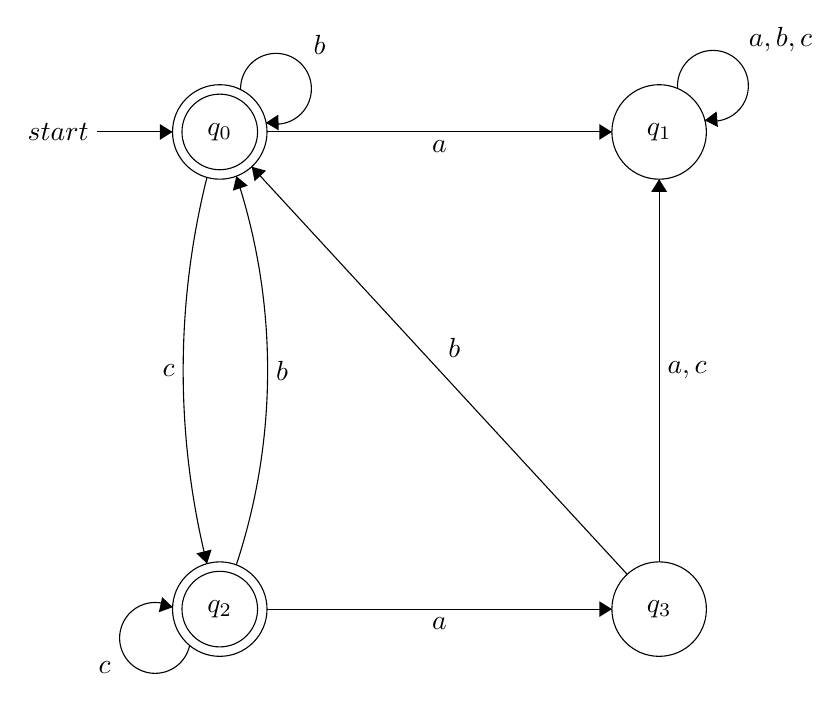
\begin{tikzpicture}[scale=0.2]
\tikzstyle{every node}+=[inner sep=0pt]
\draw [black] (17.3,-9.6) circle (3);
\draw (17.3,-9.6) node {$q_0$};
\draw [black] (17.3,-9.6) circle (2.4);
\draw [black] (45.2,-9.6) circle (3);
\draw (45.2,-9.6) node {$q_1$};
\draw [black] (17.3,-39.9) circle (3);
\draw (17.3,-39.9) node {$q_2$};
\draw [black] (17.3,-39.9) circle (2.4);
\draw [black] (45.2,-39.9) circle (3);
\draw (45.2,-39.9) node {$q_3$};
\draw [black] (9.5,-9.6) -- (14.3,-9.6);
\draw (9,-9.6) node [left] {$start$};
\fill [black] (14.3,-9.6) -- (13.5,-9.1) -- (13.5,-10.1);
\draw [black] (18.62,-6.919) arc (181.52384:-106.47616:2.25);
\draw (23.22,-4.08) node [right] {$b$};
\fill [black] (20.23,-9.02) -- (21.04,-9.5) -- (21.02,-8.5);
\draw [black] (20.3,-9.6) -- (42.2,-9.6);
\fill [black] (42.2,-9.6) -- (41.4,-9.1) -- (41.4,-10.1);
\draw (31.25,-10.1) node [below] {$a$};
\draw [black] (16.486,-37.013) arc (-165.94677:-194.05323:50.502);
\fill [black] (16.49,-37.01) -- (16.78,-36.12) -- (15.81,-36.36);
\draw (14.47,-24.75) node [left] {$c$};
\draw [black] (18.35,-12.409) arc (18.30974:-18.30974:39.282);
\fill [black] (18.35,-12.41) -- (18.13,-13.33) -- (19.08,-13.01);
\draw (20.84,-24.75) node [right] {$b$};
\draw [black] (15.39,-42.198) arc (-12.00453:-300.00453:2.25);
\draw (10.41,-43.64) node [left] {$c$};
\fill [black] (14.31,-39.78) -- (13.64,-39.13) -- (13.43,-40.1);
\draw [black] (20.3,-39.9) -- (42.2,-39.9);
\fill [black] (42.2,-39.9) -- (41.4,-39.4) -- (41.4,-40.4);
\draw (31.25,-40.4) node [below] {$a$};
\draw [black] (43.17,-37.69) -- (19.33,-11.81);
\fill [black] (19.33,-11.81) -- (19.51,-12.73) -- (20.24,-12.06);
\draw (31.78,-23.29) node [right] {$b$};
\draw [black] (45.2,-36.9) -- (45.2,-12.6);
\fill [black] (45.2,-12.6) -- (44.7,-13.4) -- (45.7,-13.4);
\draw (45.7,-24.75) node [right] {$a,c$};
\draw [black] (46.374,-6.852) arc (184.60129:-103.39871:2.25);
\draw (50.87,-3.76) node [right] {$a,b,c$};
\fill [black] (48.1,-8.86) -- (48.93,-9.29) -- (48.85,-8.3);
\end{tikzpicture}
\end{center}
\section*{Answer 3}
\subsection*{a.}
There are several possibilities in NFA, hence all of the possibilities must be computed to show a word is not in a language.
\begin{align*}
   1: (q_0, abbb) & \vdash_M (q_1, bbb) \\
   & \vdash_M (q_3, bbb) \\
   & \vdash_M (q_3, bb)\\
   & \vdash_M (q_3, b)\\
   & \vdash_M (q_3, e) [non-final]
\end{align*}
\begin{align*}
   2: (q_0, abbb) & \vdash_M (q_1, bbb) \\
   & \vdash_M (q_3, bbb) \\
   & \vdash_M (q_3, bb)\\
   & \vdash_M (q_3, b)\\
   & \vdash_M (q_4, e) [non-final]
\end{align*}
\begin{align*}
   3: (q_0, abbb) & \vdash_M (q_1, bbb) \\
   & \vdash_M (q_3, bbb) \\
   & \vdash_M (q_3, bb)\\
   & \vdash_M (q_4, b)\\
   & \vdash_M (q_3, e) [non-final]
\end{align*}
\begin{align*}
   4: (q_0, abbb) & \vdash_M (q_1, bbb) \\
   & \vdash_M (q_3, bbb) \\
   & \vdash_M (q_4, bb)\\
   & \vdash_M (q_3, b)\\
   & \vdash_M (q_3, e) [non-final]
\end{align*}
\begin{align*}
   5: (q_0, abbb) & \vdash_M (q_1, bbb) \\
   & \vdash_M (q_3, bbb) \\
   & \vdash_M (q_4, bb)\\
   & \vdash_M (q_3, b)\\
   & \vdash_M (q_4, e) [non-final]
\end{align*}
\begin{align*}
   6: (q_0, abbb) & \vdash_M (q_1, bbb) \\
   & \vdash_M (q_2, bbb) [stuck]
\end{align*}
% a q_1
\begin{align*}
    7: (q_0, abbb) & \vdash_M (q_2, abbb) \\
    & \vdash_M (q_2, abbb) [stuck]
\end{align*}
\begin{align*}
    8: (q_0, abbb) & \vdash_M (q_2, abbb) \\
    & \vdash_M (q_4, bbb)\\
    & \vdash_M (q_3, bb)\\
    & \vdash_M (q_3, b)\\
    & \vdash_M (q_3, e)[non-final]
\end{align*}
\begin{align*}
    9: (q_0, abbb) & \vdash_M (q_2, abbb) \\
    & \vdash_M (q_4, bbb)\\
    & \vdash_M (q_3, bb)\\
    & \vdash_M (q_3, b)\\
    & \vdash_M (q_4, e) [non-final]
\end{align*}
\begin{align*}
    10: (q_0, abbb) & \vdash_M (q_2, abbb) \\
    & \vdash_M (q_4, bbb)\\
    & \vdash_M (q_3, bb)\\
    & \vdash_M (q_4, b)\\
    & \vdash_M (q_3, e) [non-final]
\end{align*}
There is not any computation to start from starting state and finish with an accepting state. Hence $w1 = abbb$ is not in $L(N)$.

\subsection*{b.}
\begin{align*}
    (q_0, ababa) & \vdash_M (q_1, baba) \\
    &\vdash_M (q_3, baba) \\
    &\vdash_M (q_4, aba) \\
    &\vdash_M (q_5, ba) \\
    &\vdash_M (q_1, ba) \\
    &\vdash_M (q_3, ba) \\
    &\vdash_M (q_4, a) \\
    &\vdash_M (q_5, e)
\end{align*}
We concluded the computation with $F = \{q_5\}$, hence $w_2 = ababa$ is in $L(N)$.


\section*{Answer 4}
\subsection*{a.}
A GFA has only one starting and accepting state. Moreover, a starting state cannot be an accepting state. Hence, several trivial transitions has to be added. Set of states has to be expanded to include new states and there must be only one transition between states.\\
Let $G=(K, \Sigma, \Delta, S, F)$ be the \textit{Gneralized Finite Automaton} (GFA) for $N$.
We specify it as:
\begin{align*}
    K &= \{q_0, q_1, q_2, q_3, q_4\}\\
    \Sigma &= \{a,b\}\\
    \Delta &= \{(q_0, b, q_1), \\
        &~~~~~~(q_1, a, q_2), (q_1, e, q_3), \\
        &~~~~~~(q_2, a, q_0), (q_2, b, q_1), (q_2, b, q_2), (q_2, b, q_3), \\
        &~~~~~~(q_3, b, q1), (q_3, a, q_3),\\
        &~~~~~~(q_2, e, q_4), (q_3, e, q_4)
        \}\\
    S &= q_0 \\
    F &= q_4
\end{align*}
Note that $e$ means the empty-transition. $G$ is drawn below.

\begin{center}
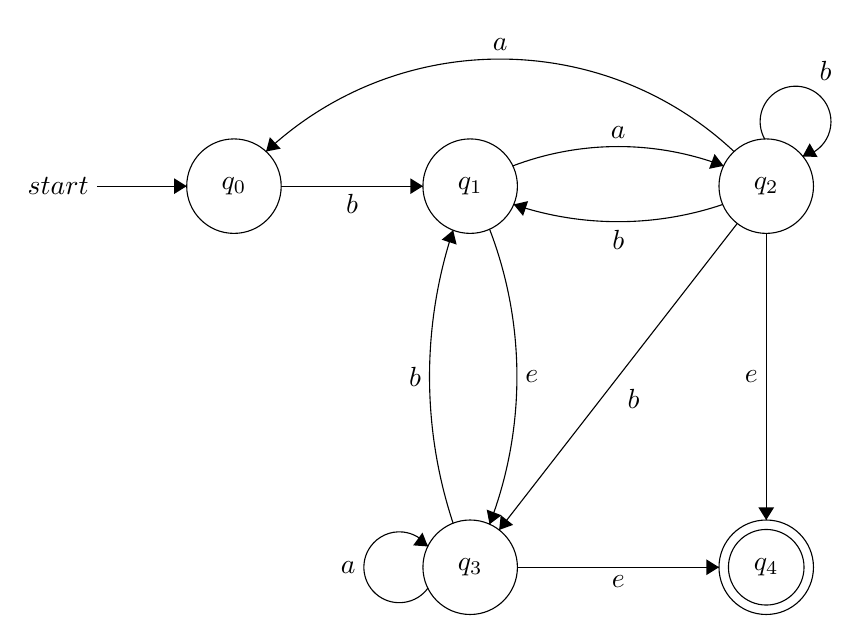
\begin{tikzpicture}[scale=0.2]
\tikzstyle{every node}+=[inner sep=0pt]
\draw [black] (31,-19.6) circle (3);
\draw (31,-19.6) node {$q_0$};
\draw [black] (46,-19.6) circle (3);
\draw (46,-19.6) node {$q_1$};
\draw [black] (46,-43.8) circle (3);
\draw (46,-43.8) node {$q_3$};
\draw [black] (64.8,-19.6) circle (3);
\draw (64.8,-19.6) node {$q_2$};
\draw [black] (64.8,-43.8) circle (3);
\draw (64.8,-43.8) node {$q_4$};
\draw [black] (64.8,-43.8) circle (2.4);
\draw [black] (34,-19.6) -- (43,-19.6);
\fill [black] (43,-19.6) -- (42.2,-19.1) -- (42.2,-20.1);
\draw (38.5,-20.1) node [below] {$b$};
\draw [black] (48.707,-18.315) arc (110.82708:69.17292:18.824);
\fill [black] (62.09,-18.31) -- (61.52,-17.56) -- (61.17,-18.5);
\draw (55.4,-16.58) node [above] {$a$};
\draw [black] (62.038,-20.764) arc (-71.30649:-108.69351:20.71);
\fill [black] (48.76,-20.76) -- (49.36,-21.49) -- (49.68,-20.55);
\draw (55.4,-22.36) node [below] {$b$};
\draw [black] (64.705,-16.613) arc (209.55605:-78.44395:2.25);
\draw (68.57,-12.95) node [above] {$b$};
\fill [black] (67.11,-17.71) -- (68.06,-17.75) -- (67.56,-16.88);
\draw [black] (62.96,-21.97) -- (47.84,-41.43);
\fill [black] (47.84,-41.43) -- (48.73,-41.11) -- (47.94,-40.49);
\draw (55.97,-33.11) node [right] {$b$};
\draw [black] (47.233,-22.333) arc (20.99839:-20.99839:26.14);
\fill [black] (47.23,-41.07) -- (47.99,-40.5) -- (47.05,-40.14);
\draw (49.47,-31.7) node [right] {$e$};
\draw [black] (44.916,-41.004) arc (-161.70918:-198.29082:29.646);
\fill [black] (44.92,-22.4) -- (44.19,-23) -- (45.14,-23.31);
\draw (42.92,-31.7) node [left] {$b$};
\draw [black] (43.32,-45.123) arc (324:36:2.25);
\draw (38.75,-43.8) node [left] {$a$};
\fill [black] (43.32,-42.48) -- (42.97,-41.6) -- (42.38,-42.41);
\draw [black] (64.8,-22.6) -- (64.8,-40.8);
\fill [black] (64.8,-40.8) -- (65.3,-40) -- (64.3,-40);
\draw (64.3,-31.7) node [left] {$e$};
\draw [black] (49,-43.8) -- (61.8,-43.8);
\fill [black] (61.8,-43.8) -- (61,-43.3) -- (61,-44.3);
\draw (55.4,-44.3) node [below] {$e$};
\draw [black] (33.04,-17.404) arc (133.14712:46.85288:21.728);
\fill [black] (33.04,-17.4) -- (33.97,-17.22) -- (33.28,-16.49);
\draw (47.9,-11.03) node [above] {$a$};
\draw [black] (22.3,-19.6) -- (28,-19.6);
\draw (21.8,-19.6) node [left] {$start$};
\fill [black] (28,-19.6) -- (27.2,-19.1) -- (27.2,-20.1);
\end{tikzpicture}
\end{center}

\subsection*{b.}
Non-final and non-initial states will be eliminated step-by-step. Starting from $q_1$, the following expressions can be found where,\\
$R(i,j,k):- $ \textit{generalized transition that moves state $q_i$ to $q_j$ using states numbered 1 to k}.\\
$R(i,j,k) = R(i,j,k-1) \cup R(i,k,k-1)R(k,k,k-1)^*R(k,j,k-1) $\\~\\
\begin{align*}
    R(0,2,1) &= ba\\
    R(0,3,1) &= b\\
    R(2,0,1) &= a\\
    R(2,2,1) &= b\cup ba\\
    R(2,3,1) &= b\cup b \text{ (which is the same as b)}\\
    R(3,2,1) &= ba\\
    R(3,3,1) &= b\cup a\\
\end{align*}
Below is the $GFA$ where $q_1$ state is eliminated.

\begin{center}
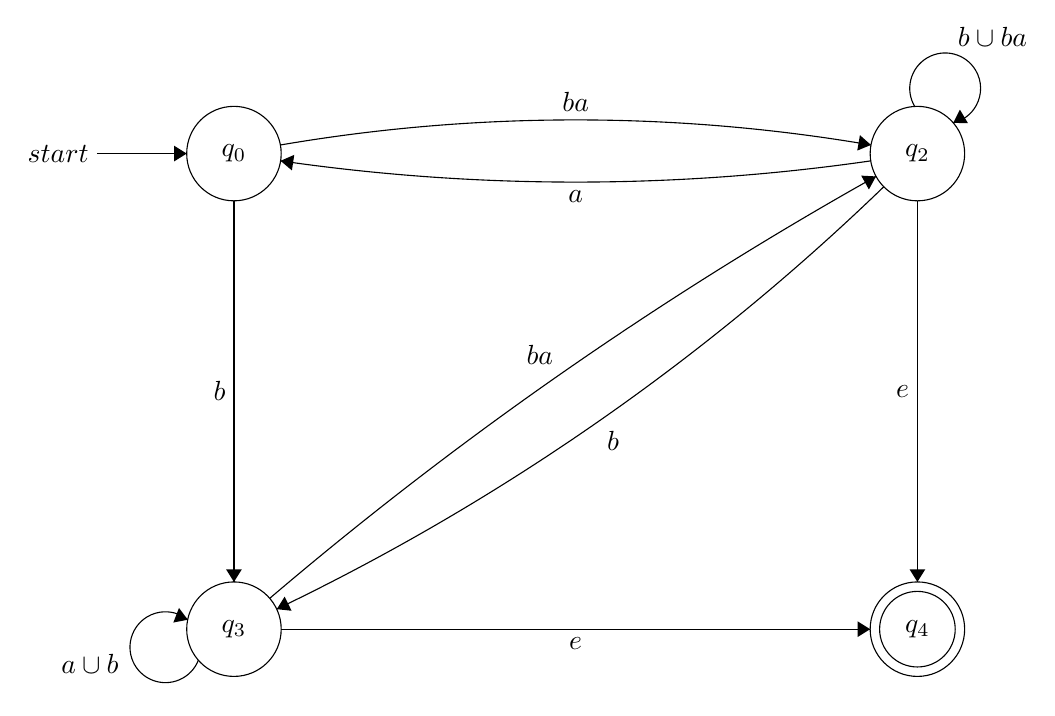
\begin{tikzpicture}[scale=0.2]
\tikzstyle{every node}+=[inner sep=0pt]
\draw [black] (19.4,-12.4) circle (3);
\draw (19.4,-12.4) node {$q_0$};
\draw [black] (19.4,-42.6) circle (3);
\draw (19.4,-42.6) node {$q_3$};
\draw [black] (62.8,-12.4) circle (3);
\draw (62.8,-12.4) node {$q_2$};
\draw [black] (62.8,-42.6) circle (3);
\draw (62.8,-42.6) node {$q_4$};
\draw [black] (62.8,-42.6) circle (2.4);
\draw [black] (62.633,-9.416) arc (210.9343:-77.0657:2.25);
\draw (67.57,-5.66) node [above] {$b\cup ba$};
\fill [black] (65.07,-10.45) -- (66.01,-10.47) -- (65.5,-9.61);
\draw [black] (60.664,-14.507) arc (-45.97879:-64.35676:147.036);
\fill [black] (22.12,-41.33) -- (23.06,-41.43) -- (22.62,-40.53);
\draw (43.47,-29.97) node [below] {$b$};
\draw [black] (17.145,-44.561) arc (-21.25375:-309.25375:2.25);
\draw (12.11,-44.81) node [left] {$a\cup b$};
\fill [black] (16.47,-42) -- (15.91,-41.25) -- (15.55,-42.18);
\draw [black] (62.8,-15.4) -- (62.8,-39.6);
\fill [black] (62.8,-39.6) -- (63.3,-38.8) -- (62.3,-38.8);
\draw (62.3,-27.5) node [left] {$e$};
\draw [black] (22.4,-42.6) -- (59.8,-42.6);
\fill [black] (59.8,-42.6) -- (59,-42.1) -- (59,-43.1);
\draw (41.1,-43.1) node [below] {$e$};
\draw [black] (59.836,-12.863) arc (-81.77154:-98.22846:130.911);
\fill [black] (22.36,-12.86) -- (23.08,-13.47) -- (23.23,-12.48);
\draw (41.1,-14.71) node [below] {$a$};
\draw [black] (10.7,-12.4) -- (16.4,-12.4);
\draw (10.2,-12.4) node [left] {$start$};
\fill [black] (16.4,-12.4) -- (15.6,-11.9) -- (15.6,-12.9);
\draw [black] (22.35,-11.854) arc (99.71942:80.28058:111.064);
\fill [black] (59.85,-11.85) -- (59.15,-11.23) -- (58.98,-12.21);
\draw (41.1,-9.76) node [above] {$ba$};
\draw [black] (19.4,-15.4) -- (19.4,-39.6);
\fill [black] (19.4,-39.6) -- (19.9,-38.8) -- (18.9,-38.8);
\draw (18.9,-27.5) node [left] {$b$};
\draw [black] (21.672,-40.641) arc (130.41299:119.25146:241.163);
\fill [black] (60.17,-13.85) -- (59.23,-13.8) -- (59.72,-14.68);
\draw (38.82,-25.81) node [above] {$ba$};
\end{tikzpicture}
\end{center}
Continuing with the elimination of $q_2$, 
\begin{align*}
    R(0,0,2) &= ba(b\cup ba)^*a\\
    R(0,3,2) &= b\cup ba(b\cup ba)^*b\\
    R(0,4,2) &= ba(b\cup ba)^*\\
    R(3,0,2) &= ba(b\cup ba)^*a\\
    R(3,3,2) &= (a\cup b)\cup (ba(b\cup ba)^*b)\\
    R(3,4,2) &= e\cup ba(b\cup ba)^*\\
\end{align*}\\~\\~\\
Below is a $GFA$ where $q_2$ is eliminated,

\begin{center}
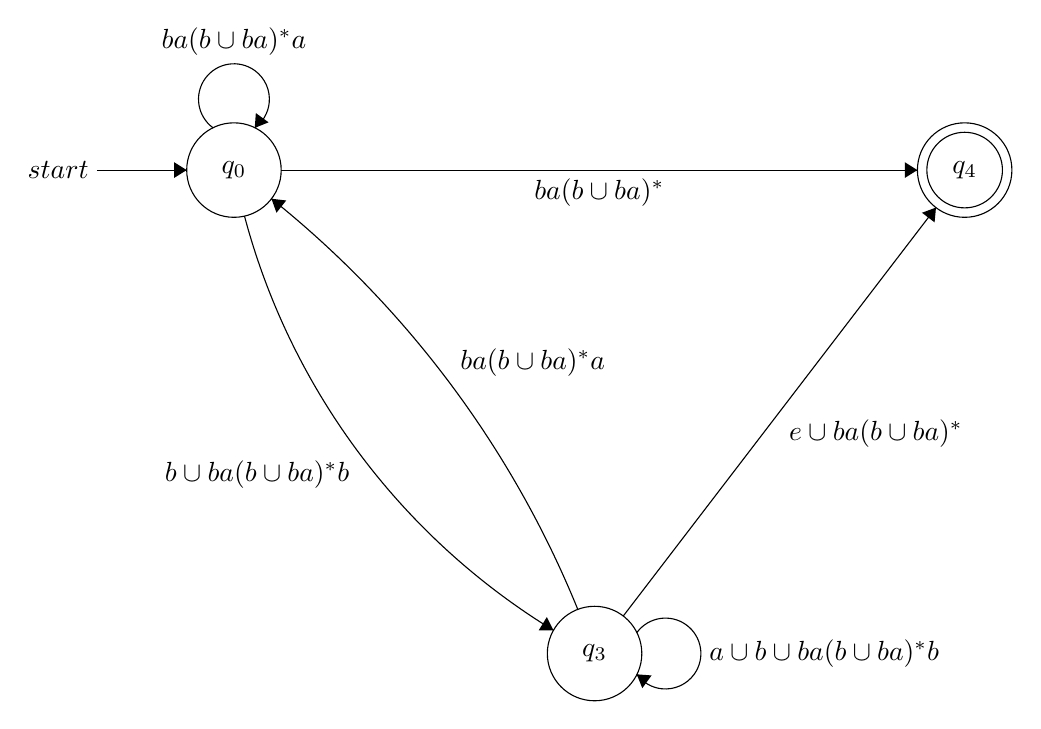
\begin{tikzpicture}[scale=0.2]
\tikzstyle{every node}+=[inner sep=0pt]
\draw [black] (19.4,-12.4) circle (3);
\draw (19.4,-12.4) node {$q_0$};
\draw [black] (42.3,-43.1) circle (3);
\draw (42.3,-43.1) node {$q_3$};
\draw [black] (65.8,-12.4) circle (3);
\draw (65.8,-12.4) node {$q_4$};
\draw [black] (65.8,-12.4) circle (2.4);
\draw [black] (44.98,-41.777) arc (144:-144:2.25);
\draw (49.55,-43.1) node [right] {$a\cup b\cup ba(b\cup ba)^*b$};
\fill [black] (44.98,-44.42) -- (45.33,-45.3) -- (45.92,-44.49);
\draw [black] (10.7,-12.4) -- (16.4,-12.4);
\draw (10.2,-12.4) node [left] {$start$};
\fill [black] (16.4,-12.4) -- (15.6,-11.9) -- (15.6,-12.9);
\draw [black] (22.4,-12.4) -- (62.8,-12.4);
\fill [black] (62.8,-12.4) -- (62,-11.9) -- (62,-12.9);
\draw (42.6,-12.9) node [below] {$ba(b\cup ba)^*$};
\draw [black] (39.689,-41.624) arc (-121.43816:-165.12124:44.096);
\fill [black] (39.69,-41.62) -- (39.27,-40.78) -- (38.75,-41.63);
\draw (26.76,-31.76) node [left] {$b\cup ba(b\cup ba)^*b$};
\draw [black] (21.784,-14.221) arc (51.28758:22.15302:64.668);
\fill [black] (21.78,-14.22) -- (22.1,-15.11) -- (22.72,-14.33);
\draw (33.75,-24.62) node [right] {$ba(b\cup ba)^*a$};
\draw [black] (18.077,-9.72) arc (234:-54:2.25);
\draw (19.4,-5.15) node [above] {$ba(b\cup ba)^*a$};
\fill [black] (20.72,-9.72) -- (21.6,-9.37) -- (20.79,-8.78);
\draw [black] (44.12,-40.72) -- (63.98,-14.78);
\fill [black] (63.98,-14.78) -- (63.09,-15.11) -- (63.89,-15.72);
\draw (54.62,-29.16) node [right] {$e\cup ba(b\cup ba)^*$};
\end{tikzpicture}
\end{center}
Continuing with the elimination of $q_3$,
\begin{align*}
    R(0,0,3) &= ba(b\cup ba)^*a\cup (b\cup ba(b\cup ba)^*b)(a\cup b\cup ba(b\cup ba)^*b)^*(ba(b\cup ba)^*a)\\
    R(0,4,3) &= ba(b\cup ba)^*(b\cup ba(b\cup ba)^*b)(a\cup b\cup ba(b\cup ba)^*b)^*(e\cup ba(b\cup ba)^*)
\end{align*}
Below is a $GFA$ where $q_3$ is eliminated,
\begin{center}
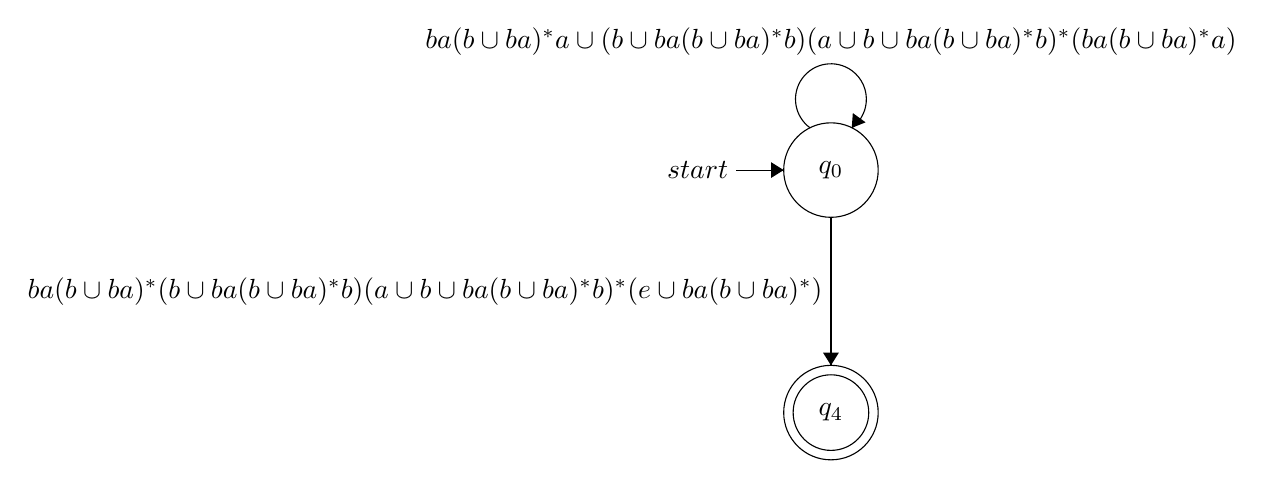
\begin{tikzpicture}[scale=0.2]
\tikzstyle{every node}+=[inner sep=0pt]
\draw [black] (40,-10.5) circle (3);
\draw (40,-10.5) node {$q_0$};
\draw [black] (40,-25.9) circle (3);
\draw (40,-25.9) node {$q_4$};
\draw [black] (40,-25.9) circle (2.4);
\draw [black] (34,-10.5) -- (37,-10.5);
\draw (33.5,-10.5) node [left] {$start$};
\fill [black] (37,-10.5) -- (36.2,-10) -- (36.2,-11);
\draw [black] (40,-13.5) -- (40,-22.9);
\fill [black] (40,-22.9) -- (40.5,-22.1) -- (39.5,-22.1);
\draw (39.5,-18.2) node [left] {$ba(b\cup ba)^*(b\cup ba(b\cup ba)^*b)(a\cup b\cup ba(b\cup ba)^*b)^*(e\cup ba(b\cup ba)^*)$};
\draw [black] (38.677,-7.82) arc (234:-54:2.25);
\draw (40,-3.25) node [above] {$ba(b\cup ba)^*a\cup (b\cup ba(b\cup ba)^*b)(a\cup b\cup ba(b\cup ba)^*b)^*(ba(b\cup ba)^*a)$};
\fill [black] (41.32,-7.82) -- (42.2,-7.47) -- (41.39,-6.88);
\end{tikzpicture}
\end{center}
Hence, the regular expression corresponding to the finite automaton is,\\
$(ba(b\cup ba)^*a\cup (b\cup ba(b\cup ba)^*b)(a\cup b\cup ba(b\cup ba)^*b)^*(ba(b\cup ba)^*a))^*\\(ba(b\cup ba)^*(b\cup ba(b\cup ba)^*b)(a\cup b\cup ba(b\cup ba)^*b)^*(e\cup ba(b\cup ba)^*))$
\section*{Answer 5}
\subsection*{a.}
Using \textit{powerset construction algorithm}, the following table can be found. Dead(trap) state is denoted by empty-set. Powerset of $\Sigma~~(2^\Sigma)$ is the new set of states.  However, not every state is reachable. Therefore, only the reachable subset of them are used. Starting from the starting state (and the states where there is an e-transition from the starting state), union of possible states is created as a new state, for each symbol in the alphabet.
\begin{table*}[!h]
\centering
\begin{tabular}{c|c|c}
 Set of States  & a       & b       \\\hline
\{0,1,2\} & \{1,3\} & \{2\}  \\\hline
\{2\}     & \{1,3\} & $\emptyset$        \\\hline
\{1,3\}   &    $\emptyset$     & \{1\}   \\\hline
\{1\}     &     $\emptyset$    &    $\emptyset$\\\hline
$\emptyset$ & $\emptyset$ & $\emptyset$
\end{tabular}
\end{table*}
\\
To formally define $D$, the DFA equivalent to N, $D = (K, \Sigma, \Delta, S, F)$,
\[
K = \{q_0, q_1, q_2, q_3, q_4\}
\]
$q_4$ is used to denote the dead(trap) state and the set of states corresponding to K is as the following,
\begin{align*}
    q_0 &\rightarrow \{0,1,2\}\\
    q_1 &\rightarrow \{2\}\\
    q_2 &\rightarrow \{1,3\}\\
    q_3 &\rightarrow \{1\}\\
    q_4 &\rightarrow \emptyset
\end{align*}
Continuing to define $D$,\\~\\
\begin{align*}
\Sigma &= \{a,b\}\\
\Delta &= \{(q_0, a, q_2), (q_0, b, q_1),\\
&~~~~~~(q_1,a,q_2), (q_1, b, q_4),\\
&~~~~~~(q_2,a,q_4),(q_2,b,q_3),\\
&~~~~~~(q_3,a,q_4),(q_3,b,q_4),\\
&~~~~~~(q_4,a,q_4),(q_4,b,q_4)\}\\
    S &= q_0\\
    F &= q_2
\end{align*}\\~\\~\\~\\
Below are two DFAs that are both using the set notation and $q_i$ notation.
\begin{center}
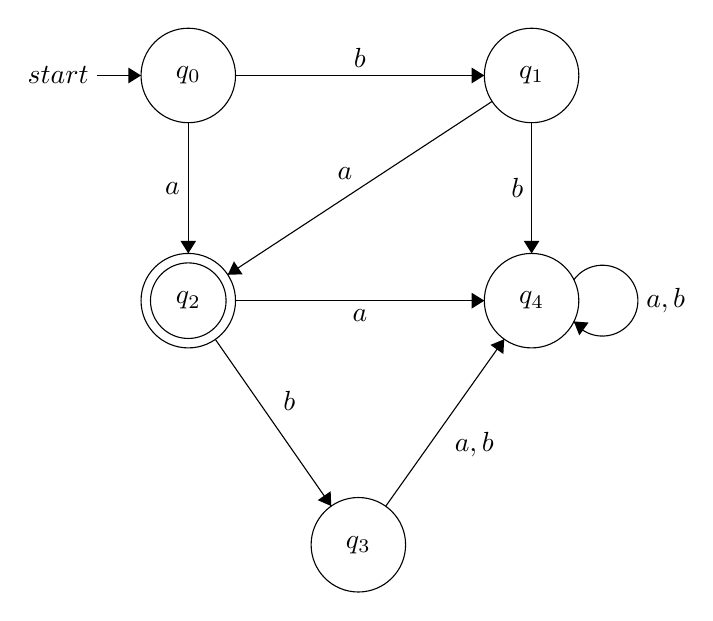
\begin{tikzpicture}[scale=0.2]
\tikzstyle{every node}+=[inner sep=0pt]
\draw [black] (11.9,-5.8) circle (3);
\draw (11.9,-5.8) node {$q_0$};
\draw [black] (33.7,-5.8) circle (3);
\draw (33.7,-5.8) node {$q_1$};
\draw [black] (11.9,-20.1) circle (3);
\draw (11.9,-20.1) node {$q_2$};
\draw [black] (11.9,-20.1) circle (2.4);
\draw [black] (22.7,-35.6) circle (3);
\draw (22.7,-35.6) node {$q_3$};
\draw [black] (33.7,-20.1) circle (3);
\draw (33.7,-20.1) node {$q_4$};
\draw [black] (36.38,-18.777) arc (144:-144:2.25);
\draw (40.95,-20.1) node [right] {$a,b$};
\fill [black] (36.38,-21.42) -- (36.73,-22.3) -- (37.32,-21.49);
\draw [black] (11.9,-8.8) -- (11.9,-17.1);
\fill [black] (11.9,-17.1) -- (12.4,-16.3) -- (11.4,-16.3);
\draw (11.4,-12.95) node [left] {$a$};
\draw [black] (14.9,-5.8) -- (30.7,-5.8);
\fill [black] (30.7,-5.8) -- (29.9,-5.3) -- (29.9,-6.3);
\draw (22.8,-5.3) node [above] {$b$};
\draw [black] (31.19,-7.45) -- (14.41,-18.45);
\fill [black] (14.41,-18.45) -- (15.35,-18.43) -- (14.8,-17.6);
\draw (21.85,-12.45) node [above] {$a$};
\draw [black] (33.7,-8.8) -- (33.7,-17.1);
\fill [black] (33.7,-17.1) -- (34.2,-16.3) -- (33.2,-16.3);
\draw (33.2,-12.95) node [left] {$b$};
\draw [black] (6.1,-5.8) -- (8.9,-5.8);
\draw (5.6,-5.8) node [left] {$start$};
\fill [black] (8.9,-5.8) -- (8.1,-5.3) -- (8.1,-6.3);
\draw [black] (14.9,-20.1) -- (30.7,-20.1);
\fill [black] (30.7,-20.1) -- (29.9,-19.6) -- (29.9,-20.6);
\draw (22.8,-20.6) node [below] {$a$};
\draw [black] (13.62,-22.56) -- (20.98,-33.14);
\fill [black] (20.98,-33.14) -- (20.94,-32.2) -- (20.12,-32.77);
\draw (17.9,-26.49) node [right] {$b$};
\draw [black] (24.44,-33.15) -- (31.96,-22.55);
\fill [black] (31.96,-22.55) -- (31.09,-22.91) -- (31.91,-23.49);
\draw (28.79,-29.22) node [right] {$a,b$};
\end{tikzpicture}
\end{center}
\begin{center}
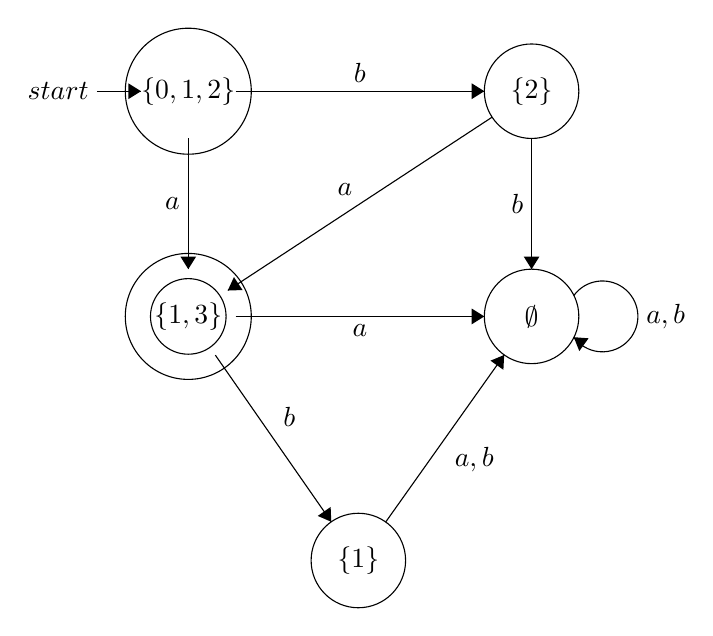
\begin{tikzpicture}[scale=0.2]
\tikzstyle{every node}+=[inner sep=0pt]
\draw [black] (11.9,-5.8) circle (4);
\draw (11.9,-5.8) node {$\{0,1,2\}$};
\draw [black] (33.7,-5.8) circle (3);
\draw (33.7,-5.8) node {$\{2\}$};
\draw [black] (11.9,-20.1) circle (4);
\draw (11.9,-20.1) node {$\{1,3\}$};
\draw [black] (11.9,-20.1) circle (2.4);
\draw [black] (22.7,-35.6) circle (3);
\draw (22.7,-35.6) node {$\{1\}$};
\draw [black] (33.7,-20.1) circle (3);
\draw (33.7,-20.1) node {$\emptyset$};
\draw [black] (36.38,-18.777) arc (144:-144:2.25);
\draw (40.95,-20.1) node [right] {$a,b$};
\fill [black] (36.38,-21.42) -- (36.73,-22.3) -- (37.32,-21.49);
\draw [black] (11.9,-8.8) -- (11.9,-17.1);
\fill [black] (11.9,-17.1) -- (12.4,-16.3) -- (11.4,-16.3);
\draw (11.4,-12.95) node [left] {$a$};
\draw [black] (14.9,-5.8) -- (30.7,-5.8);
\fill [black] (30.7,-5.8) -- (29.9,-5.3) -- (29.9,-6.3);
\draw (22.8,-5.3) node [above] {$b$};
\draw [black] (31.19,-7.45) -- (14.41,-18.45);
\fill [black] (14.41,-18.45) -- (15.35,-18.43) -- (14.8,-17.6);
\draw (21.85,-12.45) node [above] {$a$};
\draw [black] (33.7,-8.8) -- (33.7,-17.1);
\fill [black] (33.7,-17.1) -- (34.2,-16.3) -- (33.2,-16.3);
\draw (33.2,-12.95) node [left] {$b$};
\draw [black] (6.1,-5.8) -- (8.9,-5.8);
\draw (5.6,-5.8) node [left] {$start$};
\fill [black] (8.9,-5.8) -- (8.1,-5.3) -- (8.1,-6.3);
\draw [black] (14.9,-20.1) -- (30.7,-20.1);
\fill [black] (30.7,-20.1) -- (29.9,-19.6) -- (29.9,-20.6);
\draw (22.8,-20.6) node [below] {$a$};
\draw [black] (13.62,-22.56) -- (20.98,-33.14);
\fill [black] (20.98,-33.14) -- (20.94,-32.2) -- (20.12,-32.77);
\draw (17.9,-26.49) node [right] {$b$};
\draw [black] (24.44,-33.15) -- (31.96,-22.55);
\fill [black] (31.96,-22.55) -- (31.09,-22.91) -- (31.91,-23.49);
\draw (28.79,-29.22) node [right] {$a,b$};
\end{tikzpicture}
\end{center}
\subsection*{b.}
Before attempting to find the $\overline L$, it can be seen that there is a possibility to eliminate the $q_3$ state. Since $q_3$ goes to $q_4$ unconditionally (with all letters in $\Sigma$), the transitions going through $q_3$ can be merged with $(q_2,a,q_4)$. The resulting DFA is the following.
\begin{center}
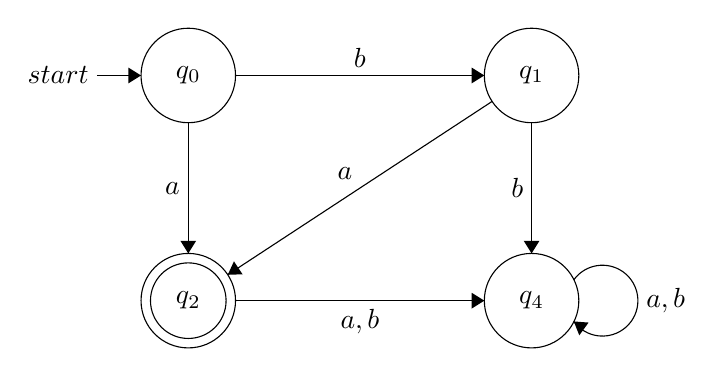
\begin{tikzpicture}[scale=0.2]
\tikzstyle{every node}+=[inner sep=0pt]
\draw [black] (11.9,-5.8) circle (3);
\draw (11.9,-5.8) node {$q_0$};
\draw [black] (33.7,-5.8) circle (3);
\draw (33.7,-5.8) node {$q_1$};
\draw [black] (11.9,-20.1) circle (3);
\draw (11.9,-20.1) node {$q_2$};
\draw [black] (11.9,-20.1) circle (2.4);
\draw [black] (33.7,-20.1) circle (3);
\draw (33.7,-20.1) node {$q_4$};
\draw [black] (36.38,-18.777) arc (144:-144:2.25);
\draw (40.95,-20.1) node [right] {$a,b$};
\fill [black] (36.38,-21.42) -- (36.73,-22.3) -- (37.32,-21.49);
\draw [black] (11.9,-8.8) -- (11.9,-17.1);
\fill [black] (11.9,-17.1) -- (12.4,-16.3) -- (11.4,-16.3);
\draw (11.4,-12.95) node [left] {$a$};
\draw [black] (14.9,-5.8) -- (30.7,-5.8);
\fill [black] (30.7,-5.8) -- (29.9,-5.3) -- (29.9,-6.3);
\draw (22.8,-5.3) node [above] {$b$};
\draw [black] (31.19,-7.45) -- (14.41,-18.45);
\fill [black] (14.41,-18.45) -- (15.35,-18.43) -- (14.8,-17.6);
\draw (21.85,-12.45) node [above] {$a$};
\draw [black] (33.7,-8.8) -- (33.7,-17.1);
\fill [black] (33.7,-17.1) -- (34.2,-16.3) -- (33.2,-16.3);
\draw (33.2,-12.95) node [left] {$b$};
\draw [black] (6.1,-5.8) -- (8.9,-5.8);
\draw (5.6,-5.8) node [left] {$start$};
\fill [black] (8.9,-5.8) -- (8.1,-5.3) -- (8.1,-6.3);
\draw [black] (14.9,-20.1) -- (30.7,-20.1);
\fill [black] (30.7,-20.1) -- (29.9,-19.6) -- (29.9,-20.6);
\draw (22.8,-20.6) node [below] {$a,b$};
\end{tikzpicture}
\end{center}
The complement of some language can be found by inverting the final and non-final states in the corresponding DFA. By inspection, it can be said that  language L accepts the regular expression $a\cup ba$ and rejects everything else. Hence, using the set notation, $\overline{L}$ accepts $\Sigma^* - (a\cup ba)$. The regular expression corresponding for that language is the following where e means the empty string.
\[
e\cup b\cup (bb\cup (a\cup ba)(a\cup b))(a\cup b)^*
\]
\section*{Answer 6}
To show the equivalence of DFA's and NFA's, it is essential to give an algorithm to demonstrate the NFA-to-DFA conversion.\\~\\
\fbox{\parbox{0.9\textwidth}{
Given an NFA $N = (K, \Sigma, \Delta, S, F)$, the equivalent DFA $D = (K', \Sigma, \Delta', S', F')$ is defined as follows:
\begin{itemize}
    \item $K' = 2^K$
    \item $S' = \delta(S,e)$
    \item $F' = \{A \subseteq K ~|~ A \cap F \neq \emptyset\}$
    \item $\Delta'(\{q_1,q_2,\dots q_i\}, a) = \delta(q_1,a) \cup \delta(q_2,a)\cup\dots\delta(q_i,a)$
\end{itemize}
$\delta(q_i,a)$ is defined as the set of states that is reachable from $q_i$ state using $a$ transition.}}\\~\\
For any two sets, we have the following identities,
\begin{align*}
    A-B &= A \cap \overline{B}\\
    \overline{\bar A} &= A\\
    A\cap B &= \overline{\overline{A}\cup\overline{B}}
\end{align*}
by De Morgan's Law. Taking two Finite Automata $F_1$ and $F_2$, they can be converted to Deterministic Finite Automata $D_1$ and $D_2$ using the algorithm given. Using the fact that they recognize $L_1$ and $L_2$ respectively, it is needed to find the following automaton. 
\[
\overline{\overline{D_1}\cup D_2}
\]
\fbox{\parbox{0.9\textwidth}{
Any individual \textit{Deterministic Finite Automaton} can be complemented using the following definition.\\
Let $D=(K,\Sigma,\Delta,S,F)$ be a DFA, then $\overline D$ is defined as,
\[
\overline D = (K, \Sigma, \Delta, S, K - F)
\]}}\\~\\
Moreover, the union of any finite automata can be constructed using the following algorithm.
\begin{itemize}
    \item Introduce a new starting state $s$
    \item Create e-transitions from $s$ to both of the previous starting states
\end{itemize}
~\\
\fbox{\parbox{0.9\textwidth}{
To give a formal definition, let $A=(K_1,\Sigma_1, \Delta_1, S_1,F_1)$ and $B = (K_2,\Sigma_2, \Delta_2, S_2,F_2)$, then
$A\cup B$ is defined as follows.
\[
A\cup B = (K_1\cup K_2\cup \{s\}, \Sigma_1\cup\Sigma_2,\Delta_1\cup\Delta_2\cup\{s,e,S_1\}\cup\{s,e,S_2\},s,F_1\cup F_2)
\]}}\\~\\
Note that this procedure yields a \textit{Nondeterministic Finite Automaton}, it may be necessary to convert it to a \textit{Deterministic Finite Automaton}, for which the algorithm is given.\\~\\
In conclusion, the required operation can be done using a series of transformations using given algorithms, with the order,
\begin{itemize}
    \item Construct DFA's for the finite automata recognizing $L_1$ and $L_2$, yielding $D_1$ and $D_2$ respectively
    \item Construct the complement of $D_1$, yielding $\overline{D_1}$
    \item Construct the union $U=\overline{D_1}\cup D_2$
    \item Convert $U$ to a DFA, yielding $M$
    \item Construct the complement of $M$, yielding $\overline M$
\end{itemize}
$\overline M$ is the automaton that recognizes $L_1-L_2$.\\~\\
Alternatively, \textit{Cross Product Construction} may also be used to create an automaton to accept $L_1-L_2$. Let $M_1=(K_1,\Sigma_1,\Delta_1,S_1,F_1)$ and $M_2=(K_2,\Sigma_2,\Delta_2,S_2,F_2)$ be DFA's to recognize $L_1$ and $L_2$, respectively. If they happen to be given as NFA's, it is not necessarily an issue since NFA's and DFA's are equivalent and an algorithm to convert NFA's to DFA's is provided. To define $M_3=(K_3,\Sigma_3,\Delta_3,S_3,F_3)$, automaton to recognize $L_1-L_2$, the following definition has to be followed.\\
\begin{align*}
    K_3 &= K_1 \times K_2 \\
    \Sigma_3 &= \Sigma_1 = \Sigma_2\\
    \Delta_3 &= ((q_i,q_j), a, (\delta(q_i,a),\delta(q_j,a)))\\
    S_3 &= (S_1,S_2)\\
    F_3 &= \{(q_i,q_j)\in K_3~|~q_i\in F_1 \text{ and } q_j\notin F_2\} 
\end{align*}
$\delta(q_i,a)$ is defined as the state that is reached by an $a$-transition from the state $q_i$. Hence, in the transition function, $\delta(q_i,a)$ moves the first element of the tuple according to the definitions in $\Delta_1$ and similarly, $\delta(q_j,a)$ moves the second element of the tuple according to the definitions in $\Delta_2$. The resulting automaton $M_3$ recognizes the language $L_1-L_2$.
\section*{Answer 7}
\subsection*{a.}
Let $p$ be some number that is to be the pumping length. The following word, $w$, is in $L$.
\[
\underbrace{(a\cup b)(a\cup b)\dots(a\cup b)}_x\underbrace{(a\cup b)(a\cup b)\dots(a\cup b)}_y\underbrace{(a\cup b)(a\cup b)\dots(a\cup b)}_z
\]
To clarify some properties about $w$,
\begin{itemize}
    \item $w=xyz$
    \item $|y| > 0$
    \item $f(a,x)=k$
    \item $f(a,y)=l$
    \item $f(a,z)=m$
    \item $k+l+m=p^2$ for some $p\in N$
    \item $f(a,w)=p^2$ for some $p \in N$
    \item $l > 0$
    \item $k+l\le p$
\end{itemize}
Since $y$ is some arbitrary substring, we can pump $y$. Let $y$ to be pumped 2 times, yielding the word $xy^2z$. Then the number of $a$'s of the string is $f(a,xy^2z)=k+2l+m=p^2+l$.\\
This string must still be in $L$ if $L$ was regular. This requires $p^2+l$ to be the square of some natural number, say $u$. However,
\begin{align*}
    (p+1)^2&=p^2+2p+1\\
    p^2+p&<p^2+2p+1\\
    p^2+l&<p^2+p\\
    p^2+l&<(p+1)^2\\
    p^2<p^2&+l<(p+1)^2\\
    p^2+l&\neq u^2
\end{align*}
$p^2+l$ is not equal to the square of any natural number. Hence, $xy^2z$ is not in $L$. Thus, $L$ is not regular by \textit{the pumping lemma}.
\end{document}